\chapter{Hidden Markov Dynamics}\label{ch:hmm}

\begin{quote}\itshape
Chapter~\ref{ch:regimes} proved that regime persistence is where
volatility clustering lives, yet every mechanism in
Chapter~\ref{ch:routing} treats each date as a fresh draw. Variation 3
closes the gap: replace the memoryless prior with a Markov chain over
regimes, and the gate becomes the predict step of a forward filter. This
chapter derives that filter from Bayes' rule, proves that its per-step
normalizers are the likelihood, draws the hard line between filtering
(admissible) and smoothing (look-ahead), and works through what it means
to train by backpropagating through the recursion. The punchline is
architectural: the entire upgrade changes one pluggable box, because the
mathematics factors exactly where the code does.
\end{quote}

\section{The model: one chain, many names}\label{sec:hmmmodel}

Let $S_t \in \{1, \dots, K\}$ be the market regime at date $t$ ---
\emph{one} latent state per date, shared by the whole cross-section, in
contrast to the memoryless model's per-sample assignments. The regime
follows a first-order Markov chain,
\[
  \Prob(S_t = k \mid S_{t-1} = j) \;=\; A_{jk},
  \qquad
  \Prob(S_1 = k) = \pi_0(k),
\]
and, given the regime, the date's cross-section is generated by that
regime's expert exactly as before:
\begin{equation}\label{eq:hmmemission}
  p(\vy_t \mid S_t = k, X_t)
  \;=\; \prod_{i \in \mathcal{U}_t}
  \gauss\!\bigl(y_{i,t};\, \mu_k(\vx_{i,t}),\, \sigma_k^2\bigr)
  \;\eqqcolon\; \ell_t(k),
\end{equation}
the \emph{per-date emission likelihood}: one number per regime per date,
aggregating the whole cross-section (in log domain, a sum of the familiar
per-name Gaussian log-densities over the date's names). The pair
(Markov prior, arbitrary emission) is a hidden Markov model; with neural
$\mu_k(\cdot)$ it is the thesis's Variation 3, and with constant
$\mu_k$ it is exactly Hamilton's model from
Chapter~\ref{ch:regimes}'s Origins box.

\section{The forward filter, derived}\label{sec:filter}

Everything an online system may know at date $t$ is $\vy_{1:t}$. Write
the \emph{filtered posterior} $r_t(k) = \Prob(S_t = k \mid \vy_{1:t})$.
It obeys a two-step recursion.

\begin{proposition}[Forward filter]\label{prop:filter}
With $\pi_t(k) \coloneqq \Prob(S_t = k \mid \vy_{1:t-1})$ (the
\emph{predictive prior}),
\begin{align}
  \text{predict:}\quad
  \pi_t(k) &= \sum_{j} A_{jk}\, r_{t-1}(j),
  \label{eq:predict}\\
  \text{update:}\quad
  r_t(k) &= \frac{\pi_t(k)\, \ell_t(k)}
                 {\sum_l \pi_t(l)\, \ell_t(l)},
  \label{eq:update}
\end{align}
initialized by $\pi_1 = \pi_0$. The cost is $O(K^2)$ per date, $O(TK^2)$
per sequence.
\end{proposition}

\begin{proof}
Predict: condition on yesterday's state and use the Markov property
($S_t \perp \vy_{1:t-1} \mid S_{t-1}$):
\[
  \Prob(S_t = k \mid \vy_{1:t-1})
  = \sum_j \Prob(S_t = k \mid S_{t-1} = j)\,
    \Prob(S_{t-1} = j \mid \vy_{1:t-1})
  = \sum_j A_{jk}\, r_{t-1}(j).
\]
Update: Bayes' rule at date $t$, with $\vy_t \perp \vy_{1:t-1} \mid S_t$
(emissions depend only on the current state):
\[
  r_t(k)
  = \frac{p(\vy_t \mid S_t = k)\, \Prob(S_t = k \mid \vy_{1:t-1})}
         {p(\vy_t \mid \vy_{1:t-1})}
  = \frac{\ell_t(k)\, \pi_t(k)}{\sum_l \ell_t(l)\, \pi_t(l)}. \qedhere
\]
\end{proof}

Now place \eqref{eq:update} next to Chapter~\ref{ch:moe}'s
responsibilities: \emph{it is the same formula}. A prior over components,
times per-component likelihoods, normalized. The only thing that changed
is where the prior comes from --- yesterday's posterior pushed through
the transition matrix, instead of a softmax of gate logits. This is the
observation the package's whole gate abstraction rests on:

\begin{engineering}[the factorization is the architecture]
The fused loss (\code{mixture\_nll}) computes ``prior + likelihood
$\to$ evidence + posterior'' without caring where the prior came from.
So the HMM upgrade touches exactly one component: a
\code{RegimePrior} whose \code{forward} implements the predict step
\eqref{eq:predict} in log domain,
\[
  \log \pi_t(k) = \LSE_j\bigl(\log r_{t-1}(j) + \log A_{jk}\bigr),
\]
consuming the previous filtered posterior through
\code{PriorContext.prev\_filtered} and marked \code{stateful = True} so
the trainer threads state chronologically. The expert bank, the
likelihood core, the loss, the diagnostics: byte-identical between
Variations 2 and 3. When mathematics factors cleanly, the highest form
of respect an implementation can pay is to factor in the same place ---
and the reward is scientific: any performance difference between the
variations is attributable to the prior mechanism, because nothing else
differs.
\end{engineering}

\section{The likelihood is the filter's by-product}
\label{sec:predictionerror}

Training needs $\log p(\vy_{1:T})$. It seems to require summing over
$K^T$ state paths; the filter has already done so.

\begin{proposition}[Prediction-error decomposition]\label{prop:preddecomp}
\begin{equation}\label{eq:preddecomp}
  \log p(\vy_{1:T})
  \;=\; \sum_{t=1}^{T} \log p(\vy_t \mid \vy_{1:t-1})
  \;=\; \sum_{t=1}^{T} \log \sum_k \pi_t(k)\, \ell_t(k):
\end{equation}
the sequence log-likelihood is the sum of the per-date log-normalizers of
the update step \eqref{eq:update}.
\end{proposition}

\begin{proof}
The first equality is the chain rule of probability. The second is the
law of total probability at date $t$ conditioned on $S_t$, with
$\Prob(S_t = k \mid \vy_{1:t-1}) = \pi_t(k)$ by definition.
\end{proof}

So the per-date training loss is $-\LSE_k(\log \pi_t(k) + \log
\ell_t(k))$ --- \emph{the same fused mixture NLL}, now with the filter's
predictive prior in the prior slot. One objective expression serves both
variations; the sum over exponentially many paths has become $T$
mixture losses chained by the recursion. Each term has a forecasting
reading worth internalizing: it is the log-score of date $t$'s
cross-section under what the model believed \emph{before seeing date
$t$} --- a strictly causal, one-step-ahead grade, which is why
maximizing \eqref{eq:preddecomp} cannot reward hindsight.

\section{Filtering versus smoothing: the causal line}
\label{sec:filtersmooth}

The filter is not the only inference the model supports. Conditioning on
the \emph{whole} sequence gives the smoothed posterior
$\Prob(S_t = k \mid \vy_{1:T})$, computed by supplementing the forward
pass with a backward recursion (Exercise~\ref{ex:7-smoother} derives
it). Smoothing is strictly better inference about $S_t$ --- it uses more
data --- and it is precisely what this project must refuse to use.

The reason is Chapter~\ref{ch:cross}'s leakage ratchet, now in state
space. The smoothed belief about date $t$ depends on returns from dates
$t+1, \dots, T$. Any prediction, position, or regime call at $t$ that
consumes a smoothed quantity has read the future --- not through a
mislabeled column this time, but through a posterior. The failure is
seductive precisely because smoothed regime paths look \emph{beautiful}:
crisp, confident, aligned with hindsight. (Every regime-model figure in
a paper that shades recessions with eerie precision is showing you a
smoother.) Filtered paths, by contrast, are visibly humbler ---
Figure~\ref{fig:hmmfilter} shows the honest product: the belief lags
each regime flip by the few days genuinely needed to distinguish signal
from one loud day, hesitates on short excursions, and that lag \emph{is
the price of causality}, not an implementation defect.

\begin{figure}[t]
  \centering
  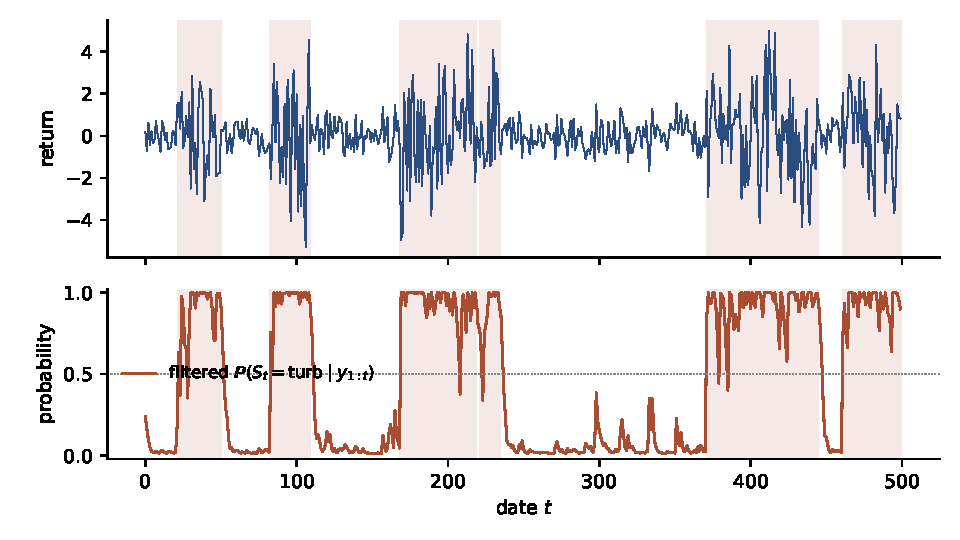
\includegraphics[width=0.9\linewidth]{figures/hmm_filter.pdf}
  \caption{\textbf{Filtering, the honest inference.} Top: returns from a
  two-state Markov scale mixture (turbulent state shaded). Bottom: the
  forward filter's $\Prob(S_t = \text{turb} \mid \vy_{1:t})$ computed
  strictly causally with the true parameters. The belief tracks every
  sustained regime but reacts with a short delay and wavers on brief
  excursions --- exactly what ``known at time $t$'' looks like. A
  smoother would clean all of this up, using data no deployable system
  has.}
  \label{fig:hmmfilter}
\end{figure}

\begin{whatbreaks}[a smoothed backtest]
Wire the smoothed posterior into a backtest --- regime-conditional
positions sized by $\Prob(S_t \mid \vy_{1:T})$ --- and regime turns are
called with hindsight's timing: the system de-risks \emph{at} the peak
and re-risks \emph{at} the trough, manufacturing a Sharpe ratio that no
live deployment can reproduce. Nothing crashes; the results are simply
fiction, and (ratchet clause) fiction in the flattering direction. The
package's defenses are structural: no smoother is implemented at all ---
\code{evaluate\_sequence} runs \eqref{eq:predict}--\eqref{eq:update}
forward only --- and the causality test perturbs future dates' data and
asserts bit-identical filtered posteriors and predictions at every
earlier date. The honest quantity is also the useful one: the
\emph{predictive} prior $\pi_t$, available before date $t$'s returns,
is what a desk would actually position on.
\end{whatbreaks}

One clarification keeps the rule precise rather than superstitious:
smoothing over the \emph{training window} during \emph{parameter
estimation} is legitimate --- classical Baum--Welch does exactly that,
and every date it smooths over lies in the past by construction. The
prohibition is on smoothed quantities crossing into prediction,
evaluation, or anything time-indexed that a deployed system would
consume. The package nonetheless trains on the filtered objective too
(next section), for reasons of its own.

\section{Training through the filter}\label{sec:bptt}

Two estimation routes exist for HMM parameters.

\emph{Route 1: Baum--Welch} --- EM instantiated for chains. E-step:
forward--backward smoothing yields state marginals and transition
pair-marginals over the training window. M-step: closed-form reestimates
of $A$ (expected transition counts) and, for \emph{Gaussian} emissions,
of $(\mu_k, \sigma_k)$ by smoothed-weighted moments. Elegant, monotone
(Theorem~\ref{thm:em} applies), and the classical choice --- but the
M-step's closed forms die the moment $\mu_k(\cdot)$ is a network, which
would leave EM's outer loop wrapped around an inner SGD anyway.

\emph{Route 2: direct gradient on the filtered NLL} --- Decision C.
Treat \eqref{eq:preddecomp} as a loss and let autograd differentiate
through the recursion itself: the predict step is a
$\LSE$ over yesterday's \emph{attached} log-posterior, so the chain rule
flows from date $t$'s loss back through $r_{t-1}, r_{t-2}, \dots$ into
every parameter --- the transition logits accumulate credit for how
\emph{beliefs they shaped days ago} paid off today. (In the classical
literature this is the ``recursive score'' computation; automatic
differentiation delivers it for free.) The package takes Route 2 for
every emission type: one optimizer, one code path shared with
Variation 2, neural emissions welcome, and the trained objective is the
same strictly-causal score the evaluation grades --- an alignment
Baum--Welch does not offer.

The practical cost is the usual cost of backpropagating through time:
memory and gradient conditioning over long sequences. The trainer
therefore chunks: within a chunk of $C$ dates the state is threaded
attached (full gradient flow); at chunk boundaries the carried posterior
is \code{detach()}ed --- truncated BPTT over the regime posterior, with
the truncation length an explicit config knob rather than a hidden
constant. Two engineering clauses follow from the mathematics. The
recursion's correctness depends on \emph{chronological, complete
per-date batches} --- shuffled minibatches would feed the filter
scrambled time --- so the stateful path validates its input ordering and
the memoryless \code{train\_step} refuses stateful priors outright.
And the carried state is part of training state: Chapter~10's
checkpointing persists the chunk cursor and carried posterior precisely
so a resumed run continues the recursion bit-exactly.

\section{Parameterizing the transition matrix}\label{sec:transition}

$A$ must be a stochastic matrix (rows on the simplex). Constrained
optimization is the wrong tool at this scale; the package uses the
standard unconstrained parameterization
\[
  A \;=\; \operatorname{row\_softmax}(L),
  \qquad L \in \R^{K \times K}\ \text{free},
\]
so any gradient step on $L$ yields a valid $A$. Two choices ride on top,
both traceable to Part I mathematics:

\emph{Persistence-biased initialization.} $L$ starts as
$\beta_{\mathrm{diag}} I$ (default bias $2$), making $A$'s diagonal
dominant from step one: with $K = 2$,
$A_{kk} = \sigma(\beta_{\mathrm{diag}}) \approx 0.88$ initial stay
probability. Chapter~\ref{ch:regimes} estimated real regime persistence
at $\lambda \approx 0.9$--$0.98$; starting the chain sticky encodes that
prior belief and --- more practically --- keeps early training out of
the fast-mixing region where the filter's beliefs slosh datewise and the
emission gradients are noise. It is the transition-matrix analogue of
initializing an LSTM's forget-gate bias positive, and like all
initializations it is a starting point, not a constraint: the data can
unlearn it.

\emph{No weight decay on $L$.} Generic weight decay shrinks parameters
toward zero; $L \to 0$ means $A \to$ \emph{uniform} --- decay would
actively pull the chain toward forgetting its own persistence, silently
fighting the initialization and the data. The trainer's parameter
groups therefore exempt prior parameters (and $\log\sigma$, for the
analogous reason) from decay. A regularizer is a prior; applying one
that contradicts the model's actual prior belief is not hygiene, it is
sabotage --- one more instance of the book's running rule that defaults
are decisions.

\section{Label permutation across refits}\label{sec:permutation}

The HMM likelihood, like every mixture's, is invariant under relabeling
the states (permute $\pi_0$, rows and columns of $A$, and the emission
parameters together). Within one training run this is harmless ---
gradient descent stays in one labeling basin. Across \emph{independent
refits} --- one per walk-forward window (Decision D), one per seed ---
it is a real hazard: window 3's ``regime 1'' may be window 4's
``regime 2,'' and any cross-window aggregation of per-regime quantities
(mean utilization of the turbulent expert, say) silently averages apples
with oranges. The repair is declared, not discovered: the package's
canonical order sorts experts by $\sigma_k$ ascending after every fit,
records the permutation per fold, and all cross-fit reporting uses
canonical indices. Chapter~\ref{ch:symmetry} folds this into the
broader identifiability picture.

\begin{codewalk}[nec\_moe/priors.py --- the predict step]
The entire Variation-3 mechanism is one \code{forward}:
\begin{lstlisting}
def forward(self, gate_logits, ctx=None):
    log_a = self.log_transition()            # (K, K) row log-softmax of L
    if ctx is None or ctx.prev_filtered is None:
        log_prior = F.log_softmax(self.pi0_logits, 0).expand(b, -1)
    else:                                    # predict step, log domain:
        log_prior = torch.logsumexp(         # LSE_j(log r_{t-1,j} + log A_jk)
            ctx.prev_filtered.unsqueeze(2) + log_a.unsqueeze(0), dim=1)
    return PriorOutput(log_prior=log_prior, ...)
\end{lstlisting}
Read it against \eqref{eq:predict}: the broadcast adds yesterday's
log-posterior (column) to $\log A$ (matrix) and $\LSE$s over the source
state --- matrix--vector multiplication in log space, numerically safe
for beliefs as confident as the data makes them. Sequence starts fall
back to $\pi_0$. Note what is \emph{absent}: no gate-logit dependence
(the encoder is dormant in the static-transition variant --- its return
would be the guarded-off time-varying-transition extension), and no
backward pass anywhere in the file. The trainer's side is
\code{train\_step\_sequence}: thread state attached within a chunk,
\code{state.detach()} at the boundary, loss = mean per-date fused NLL
--- Proposition~\ref{prop:preddecomp} rendered as a \code{for} loop.
\end{codewalk}

\exercisehead

\begin{exercise}\label{ex:7-smoother}
Derive the backward recursion: define $\beta_t(k) = p(\vy_{t+1:T} \mid
S_t = k)$, show $\beta_t(j) = \sum_k A_{jk}\, \ell_{t+1}(k)\,
\beta_{t+1}(k)$ with $\beta_T \equiv 1$, and conclude the smoothed
marginal is $\Prob(S_t = k \mid \vy_{1:T}) \propto r_t(k)\beta_t(k) /
\pi$ (state the exact normalization). Verify that computing it requires
the full future --- the formal content of ``smoothing is look-ahead.''
\end{exercise}

\begin{exercise}\label{ex:7-counter}
Construct the smallest possible counterexample to ``filtered $=$
smoothed'': $T = 2$, $K = 2$, symmetric sticky $A$, and emissions where
date 2 is loud. Compute $r_1$ and $\Prob(S_1 \mid \vy_{1:2})$ by hand
and show date 2's observation moves the belief about date 1. Then say
in one sentence what a backtest that positions at date 1 using the
latter quantity has done.
\end{exercise}

\begin{exercise}\label{ex:7-gradA}
Differentiate one step of the filtered objective with respect to the
transition logits: for the per-date loss $-\log\sum_k \pi_t(k)\ell_t(k)$
with $\pi_t$ from \eqref{eq:predict} and $A = \operatorname{row\_softmax}
(L)$, show the gradient with respect to $L_{jk}$ is
$-r_{t-1}(j)\bigl(r_t(k) - A_{jk}\,[\text{norm.\ terms}]\bigr)$-shaped
--- derive the exact expression --- and interpret: transitions are
reinforced in proportion to yesterday's belief in the source state times
today's posterior surprise in the destination. Where does
Theorem~\ref{thm:pir}'s $\pi - r$ pattern reappear?
\end{exercise}

\begin{exercise}\label{ex:7-hamilton}
Show that with \code{ClassicalGaussianEmission} (constant $\mu_k,
\sigma_k$), the filtered objective \eqref{eq:preddecomp} is exactly the
likelihood Hamilton (1989) maximized, and that the package's
parameter-recovery test --- generate from a known sticky two-state
scale mixture, fit \code{classical} $\times$ \code{hmm}, compare
$\hat A$ and $\hat\sigma$ --- is a Hamilton replication on synthetic
data. Why is rank-IC structurally meaningless for this emission
(Chapter~\ref{ch:cross}'s grading vocabulary), and what is graded
instead?
\end{exercise}

\begin{exercise}\label{ex:7-numpy}
(Hands-on.) Implement the log-domain forward filter in $\le 20$ lines of
numpy. Generate a sticky two-state panel with the package's synthetic
generator, run your filter with the \emph{true} parameters, and compare
against \code{Trainer.evaluate\_sequence}'s \code{log\_filtered} on the
same data (after loading the true parameters into a
\code{classical} $\times$ \code{hmm} model): they should agree to
numerical precision. Then break causality on purpose --- flip the sign
of the last date's returns --- and verify your filtered path before
that date is unchanged, bit for bit. You have just reimplemented the
package's causality test.
\end{exercise}

\begin{exercise}\label{ex:7-chunk}
Truncated BPTT with chunk length $C$ zeroes gradient flow across
boundaries. (a) Argue that the \emph{filter values} are unaffected ---
truncation changes gradients, never the forward computation.
(b) Identify which parameter's learning is most damaged by small $C$
(the answer moves through multi-date credit assignment), and design a
synthetic experiment that would expose it: what would you plant, and
what would you measure as a function of $C$? (c) Explain why
mean-per-date (not sum) chunk losses keep gradient magnitudes comparable
across unequal final chunks.
\end{exercise}
